\documentclass[12pt]{article}
\usepackage{amsmath}
\usepackage{amssymb}
\usepackage{cancel}
\usepackage{enumitem}
\usepackage{esdiff}
\usepackage{graphicx}
\usepackage{siunitx}
% \usepackage{pgfplots}
\usepackage{wrapfig}

\newcommand{\E}[1]{\times 10^{#1}}

\title{
    Worksheet \#8
    \\  \small
    PHYS 4C: Waves and Thermodynamics
    }
\author{Donald Aingworth IV}
\date{October 20, 2025}

\begin{document}
    \DeclareSIUnit{\celsiusdegree}{C^\circ}
    \DeclareSIUnit{\atm}{ atm}

    \maketitle

    \setcounter{section}{0}
    \section{Problem 1}
        The speed of sound in steel is 5941\,\unit{\meter/\second}.
        Steel has a density of around 7900\,\unit{\kilo\gram/\meter^3} (depends somewhat on the alloy content).
        
        a. Based on this information, what is the bulk modulus of steel?

        \begin{wrapfigure}{r}{0.25\textwidth}
            % \vspace{-30pt}
            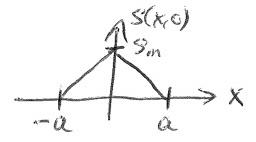
\includegraphics[width=0.25\textwidth]{4c-wspic-1617B.jpg} 
        Sound pulse graph
            % \label{fig:wrapfig}
        \end{wrapfigure}
        b. A steel rod of cross-sectional area A is placed on the x-axis.  
        The following sound pulse is sent through the steel rod in the +$x$ direction:
        
        $f(x) = s(x,0) = s_m(1 - |x|/a)$, if $|x| < a$.
        
        $f(x) = s(x,0) = 0$, if $|x| \geq a$.

        % 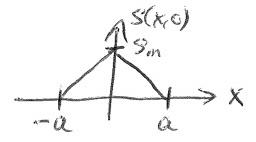
\includegraphics{4c-wspic-1617B.jpg}
        
        Determine the total energy of this pulse.
        
        c. Now suppose a sinusoidal sound wave with frequency $440\,\unit{\hertz}$ is sent through steel with a sound level of $100\,\unit{\deci\bel}$.  
        Calculate $s_m$ and $\Delta p_m$ for this sound wave.

        \subsection{Solution (a)}
            The bulk modulus is used as part of an equation for the velocity.
            \begin{equation}
                v   =   \sqrt{\frac{B}{\rho}}
            \end{equation}

            This can be solved for the bulk modulus.
            \begin{equation}
                B   =   \rho v^2
            \end{equation}

            We know all the values necessary, so we can solve this equation.
            \begin{equation}
                B   =   (7900\,\unit{\kilo\gram/\meter^3}) (5941\,\unit{\meter/\second})^2
                    =   \boxed{2.788\E{11}\,\unit{\kilo\gram/\meter\cdot\second^2}}
            \end{equation}
        
        \subsection{Solution (b)}
            If this is the initial point, there is no motion, so $\diff{s}{t} = 0$ at all points.
            There is an equation for the potential energy.
            \begin{align}
                dU  &=  \frac{1}{2} B \left( \diffp{s}{x} \right)^2 A\,dx
            \end{align}

            At time $t = 0$, the partial derivative of $s$ is calculatable, but it would have to be divided into two cases ($x \geq 0$ and $x < 0$).
            For the case of $x \geq 0$:
            \begin{align}
                \diffp{s}{x}    &=  \diffp{}{x}\left( s_m \left( 1 - \frac{x}{a} \right) \right)
                    =   -\frac{s_m}{a}
            \end{align}

            For the case of $x < 0$:
            \begin{align}
                \diffp{s}{x}    &=  \diffp{}{x}\left( s_m \left( 1 + \frac{x}{a} \right) \right)
                    =   \frac{s_m}{a}
            \end{align}

            Since the negative is the only thing differentiating these, it is safe to say that $\left( \diffp{s}{x} \right)^2$ is identical for both.

            These in turn can be plugged into our equation for the potential energy.
            \begin{align}
                dU  &=  \frac{1}{2} B \frac{s_m^2}{a^2} A\,dx
            \end{align}

            This in turn can be integrated between $-a$ and $a$.
            Technically, we would be integrating between $-\infty$ and $\infty$, but since $s(x,0) = 0$ everywhere outside the range of $(-a,a)$, all the other spots would result in zero to begin with.
            \begin{align}
                \int_{-\infty}^{\infty}\,dU &=  \int_{-\infty}^{\infty} \frac{1}{2} BA \frac{s_m^2}{a^2}\,dx\\
                U   &=  \int_{-a}^{a} \frac{1}{2} BA \frac{s_m^2}{a^2}\,dx
                    =   \frac{1}{2} BA \frac{s_m^2}{a^2}\int_{-a}^{a}\,dx\\
                    &=  \frac{1}{2} BA \frac{s_m^2}{a^2} \left[ x \right]_{-a}^{a}
                    =   \frac{1}{2} BA \frac{s_m^2}{a^2} (a - (-a))
                    =   \boxed{BA \frac{s_m^2}{a}}
            \end{align}

        \subsection{Solution (c)}
            We know the sound level.
            This can be used to calculate the intensity.
            \begin{gather}
                \beta   =   100\,\unit{\deci\bel}
                    =   (10\,\unit{\deci\bel})\,\log_{10}\frac{I}{I_0}\\
                10  =   \log_{10}\frac{I}{I_0}\\
                10^{10} =   \frac{I}{10^{-12}\,\unit{\watt/\meter^2}}\\
                10^{10} * 10^{-12}  =   10^{-2}\,\unit{\watt/\meter^2}
                    =   I
            \end{gather}
            
            Next, we know the bulk modulus ($B$), the speed of sound ($v$), and the frequency ($f$).
            The latter can be turned into the angular speed ($\omega$) by arithmetic.
            \begin{align}
                \omega = 2\pi f
            \end{align}

            We have an equation for the intensity that includes all of these values and the displacement amplitude, the latter of which can be solved for.
            \begin{gather}
                I   =   \frac{1}{2}\rho v \omega^2 s_m^2\\
                \begin{align}
                    s_m &=  \sqrt{\frac{2I}{\rho v \omega^2}}
                        =   \sqrt{\frac{2I}{\rho v (2\pi f)^2}}
                        =   \sqrt{\frac{I}{2\rho v (\pi f)^2}}\\
                        &=  \sqrt{\frac{10^{-2}\,\unit{\watt/\meter^2}}{2(7900\,\unit{\kilo\gram/\meter^3}) (5941\,\unit{\meter/\second}) (\pi * 440\,\unit{\hertz})^2}}\\
                        &=  \boxed{7.47\E{-9}\,\unit{\meter}}
                \end{align}
            \end{gather}

            The pressure amplitude is calculatable similarly.
            \begin{align}
                \Delta p_m  &=  (v \rho \omega) s_m\\
                    &=  (5941\,\unit{\meter/\second}) (7900\,\unit{\kilo\gram/\meter^3}) (2\pi * 440\,\unit{\hertz}) (7.47\E{-9}\,\unit{\meter})\\
                    &=  \boxed{968.85\,\unit{\pascal}}
            \end{align}
        
    \section{Problem 2}
        A half-open organ pipe is tuned to A(440) (i.e., the fundamental frequency is $440\,\unit{\hertz}$).
        Air has a density of $1.21\,\unit{\kilo\gram/\mole}$ and a speed of sound of $343\,\unit{\meter/\second}$ at $20\unit{\celsius}$.
        
        \begin{enumerate}[label=\alph*.]
            \item   What is the length of the pipe?
            \item   What is the maximum kinetic energy density (per unit volume) at the open end of the pipe if $s_m = 2.0\,\unit{\micro\meter}$?  At the closed end?
            \item   If the ambient temperature were raised from 20\unit{\celsius} to 40\unit{\celsius}, what would be the new fundamental frequency of the pipe (ignore changes in the length of the pipe due to the temperature change)?
        \end{enumerate}
    




\end{document}